\documentclass[popl.tex]{subfiles}
\begin{document}

\clearpage\section{Evaluation}\label{sec:eval}

We call our method Tidyparse and consider the following research questions:

\begin{itemize}
\item \textbf{RQ 1}: What statistical properties do human repairs exhibit? (e.g., length, edit distance)
\item \textbf{RQ 2}: How performant is Tidyparse at fixing syntax errors? (i.e., vs. Seq2Parse and BIFI)
\item \textbf{RQ 3}: Which design choices are most significant? (e.g., decoding, reranking, parallelism)
\end{itemize}

We address \textbf{RQ 1} in \S~\ref{sec:rq1} by analyzing the distribution of natural code snippet lengths and edit distances, \textbf{RQ 2} in \S~\ref{sec:rq2} by comparing Tidyparse against two existing syntax repair baselines, and \textbf{RQ 3} in \S~\ref{sec:rq3} by ablating various design choices and evaluating the impact on precision and latency.

\subsection{Experimental setup}

In the following set of experiments, we use syntax errors and fixes from the Python language. Python code snippets are abstracted as a sequence of lexical tokens using the official Python 3.8.11 parser, erasing alphanumeric identifiers and literals but retaining all other keywords. Accuracy is evaluated across a test set of pairwise errors and repairs by checking for lexical equivalence with the ground-truth repair, following the same methodology as Sakkas et al. (2022)~\cite{sakkas2022seq2parse}.

We use the Precision@k statistic, which measures the frequency of the true repair appearing in the top-$k$ results, across a dataset of repair instances. Specifically, given a repair model, $R: \Sigma^* \rightarrow (\Sigma^*)^t$ and a test set, $\mathcal{D}_{\text{test}}$, containing pairwise aligned errors ($\err\sigma$) and fixes ($\sigma'$), we define Precision@k as:\vspace{-0.1cm}

\begin{equation}
\text{Precision@k}(R) = |\mathcal{D}_{\text{test}}|^{-1}\sum_{\mathcal{D}_{\text{test}}} \mathds{1}\left[\sigma' \in R(\err\sigma)_{0\ldots k}\right]
\end{equation}

Our full dataset~\cite{wong2019syntax} consists of $2\times 10^4$ naturally-occurring pairs of Python errors and human fixes from StackOverflow, which we use to evaluate the precision of each model at blind recovery of the ground truth repair. From the StackOverflow dataset, we filter for syntax errors shorter than 80 tokens and fewer than four lexical edits apart from the corresponding repair, then divide the remaining repairs into two disjoint sets: a training set $(\mathcal{D}_{\text{train}})$ of 4,586 repair instances and a test set $(\mathcal{D}_{\text{test}})$ of 2,238 repair instances, balanced across each length interval and edit distance, i.e., $\mathcal{D}_{\text{test}} = \{\langle\err\sigma, \sigma'\rangle \mid \lfloor |\err\sigma|/10 \rfloor \in [0, 8], \Delta(\err\sigma, \sigma') \in [1, 3]\}$, each test bin containing at least 50 instances.

To train the reranker, we augment each instance in the training and test set with a list of repair confounders. Each instance consists of a tuple, $\langle\err\sigma: \bar{\ell}, \sigma': \ell_\cap, \bm{\sigma}: \ell_\cap^{\leq 10^3}\rangle$, with a single syntax error $(\err\sigma)$, the ground truth repair, $(\sigma')$, and up to $10^3$ confounders $(\bm{\sigma})$ sampled without replacement from $\ell_\cap$ using our pretrained $4$-gram model. We then train the reranker on $\mathcal{D}_{\text{train}}$ for 13,000 steps which takes $\sim 4$ hours, and evaluate on $\mathcal{D}_{\text{test}}$. Hyperparameters are provided in Appendix~\ref{sec:hyperparams}.

For our final repair procedure, we use the CNF Python grammar, $G_{\text{Python}}$ and let $d_{\max}$ be the smallest value such that $\ell_\cap = \mathcal{L}(G)\cap\mathcal{L}\big(L(\err\sigma, d_{\max} - 1)\big)$ is nonempty. We decode $\ell_\cap$ with the same pretrained $4$-gram model used in reranker training, and pass the top-$10^3$ results by 4-gram probability to the transformer encoder, then finally rerank the top-$10^3$ by softmax probability and measure the Precision@k across repairs of differing length and edit distance in the test set.

We compare our method with two external baselines, Seq2Parse and Break-It-Fix-It (BIFI)~\cite{yasunaga2021break}, on the same test set. The Seq2Parse and BIFI experiments were conducted on a single Nvidia V100 GPU with 32 GB of RAM. For Seq2Parse, we use the default pretrained model provided in commit \texttt{7ae0681}.~\footnote{https://github.com/gsakkas/seq2parse/tree/7ae0681f1139cb873868727f035c1b7a369c3eb9} For BIFI, we use the Round 2 breaker and fixer from commit \texttt{ee2a68c},\footnote{https://github.com/michiyasunaga/BIFI/tree/ee2a68cff8dbe88d2a2b2b5feabc7311d5f8338b} the highest-performing model reported by the authors, with a variable-width beam search to control the number of predictions, and let the BIFI fixer model predict the top-$\{1, 2\times 10^4\}$ repairs. Finally, for Tidyparse, we use a standard Apple MacBook M4 Max with 128 GB of memory.

\clearpage\subsection{Dataset statistics}\label{sec:rq1}

In the following experiments, we use a dataset of Python snippets consisting of 20,500 pairwise-aligned human errors and fixes from StackOverflow~\cite{wong2019syntax}. We preprocess the dataset to lexicalize all code snippets, then filter by length and distance shorter than 80 lexical tokens and under four edits, i.e., with Levenshtein distance under four lexical edits $\big(|\Sigma| = 88, |\err{\sigma}| < 80, \Delta(\err{\sigma}, \sigma') < 4\big)$. We depict the length, edit distance, normalized edit locations and stability profile in Fig.~\ref{fig:patch_stats}.\vspace{-0.2cm}

\begin{figure}[h!]
\input{repair_statistics}
\vspace{-0.2cm}
\caption{Repair statistics across the StackOverflow dataset, of which Tidyparse can handle about half in under $\sim$3s and $\sim$4 GB. Larger repairs and edit distances are possible, albeit requiring additional time and memory.}\label{fig:patch_stats}\vspace{-0.2cm}
\end{figure}

We observe that slightly over 6,700 code snippet pairs in the StackOverflow dataset contain fewer than 80 tokens and four lexical edits, which are computationally feasible to process in a few hundred milliseconds. We also note a slight primacy or recency bias in the edit locations, evidenced by a large fraction of human repairs which modify the boundaries of the broken code snippet.

For the stability profile, we enumerate repairs for each syntax error and estimate the average fraction of all edit locations that were never altered by any repair in the $L\big(\err\sigma, \Delta(\err\sigma, \sigma')\big)$-ball. For example, on average roughly half of the string is stable for 3-edit syntax repairs in the $[10-20)$ token range, whereas 1-edit repairs of the same length could modify only $\sim 10\%$ of all locations. For a fixed edit distance, we observe an overall decrease in the number of degrees of caret freedom with increasing length, which intuitively makes sense, as the repairs are more heavily constrained by the surrounding context and their locations grow more concentrated relative to the entire string.

\begin{wrapfigure}{r}{0.45\textwidth}
\vspace{-0.4cm}
\resizebox{.45\textwidth}{!}{\input{figures/volumetric_plot}}
\vspace{-0.8cm}
\caption{Language volume versus snippet length and edit distance for Python repairs.}
\label{fig:volumetric_plot}
\vspace{-0.2cm}
\end{wrapfigure}

For an intuition about the size of the language intersections involved in syntax repair, volumetric analysis will be helpful, particularly in understanding the influence of snippet length and edit distance on language intersection volume. To measure the intersection volume we will form the $L\big(\err\sigma, \Delta(\err{\sigma}, \sigma')\big)$ automaton, intersect it with the Python grammar, then automatize the resulting regular expression and finally compute the DFA transfer matrix using the method described in \S~\ref{sec:transfer_method} to obtain the exact volume. For a given (error, fix) pair, this tells us how many repairs of equal or lesser distance exist in the Python language. Plotting intersection volume across the full dataset (Fig.~\ref{fig:volumetric_plot}), we observe a strong positive correlation with the Levenshtein margin and a mild correlation with snippet length. Fully materializing $\ell_\cap$ is typically only feasible if we extend the Levenshtein radius up to one edit beyond the language edit distance (LED) $\big(\text{i.e., } d_{\max} \leq \text{LED}(\err\sigma)$\footnote{Where $\text{LED}(\err\sigma)$ is shorthand for $\text{LED}(\err\sigma, \ell) = \min \big\{d_{\max}: \mathbb{N}\mid \mathcal{L}\big(L(\err\sigma, d_{\max})\big) \cap \ell \neq \varnothing\big\}$ with $\ell$ being the Python language.}$+ 1\big)$ after which it grows too large to exhaustively generate and must be sampled. Across all snippets where $\Delta(\err{\sigma}, \sigma') < 4$, approximately 54\% matched $\text{LED}(\err\sigma)$, 35\% had an edit distance of $\text{LED}(\err\sigma) + 1$ and 11\% had a distance of $\text{LED}(\err\sigma) + 2$.

\clearpage\subsection{StackOverflow evaluation}\label{sec:rq2}

For our first experiment, we measure the top-1 precision of our repair procedure at various lengths and Levenshtein distances, comparing Tidyparse against Seq2Parse, and BIFI on the same test set. Each bin in the test set contains at least 50 distinct repairs sampled uniformly at random from the StackOverflow dataset, none of which were present in the training set of any repair model.\vspace{-0.2cm}

\begin{figure}[h!]
\resizebox{.29\textwidth}{!}{\begin{tikzpicture}
  \begin{axis}[
    legend cell align={left},
    legend style={fill opacity=0.8, draw opacity=1, text opacity=1, draw=lightgray204, legend columns=-1, legend pos=north east},
    xlabel={Snippet length, $|\sigma|$},
    ylabel={Precision@1},
    title={\Large\textbf{Tidyparse Repair Precision@1}},
    ybar,
    axis lines*=left,
    xtick={0, 10, 20, 30, 40, 50, 60, 70},
    ytick={0, 0.1, 0.2, 0.3, 0.4, 0.5, 0.6, 0.7, 0.8, 0.9, 1.0},
    xticklabels={{(}0{,}10{)}, {[}10{,}20{)}, {[}20{,}30{)}, {[}30{,}40{)}, {[}40{,}50{)}, {[}50{,}60{)}, {[}60{,}70{)}, {[}70{,}80{)}},
    x tick label style={font=\scriptsize},
    ymax=1.0,
    ymin=0.0,
    ymajorgrids=true,
    grid style=dashed,
    tick align=outside,
    tick pos=left,
    bar width=4pt,
  ]
  \addlegendimage{empty legend}
  \addlegendentry{$\Delta(\err\sigma, \sigma^\star)=$}
  \addlegendimage{ybar,ybar legend,draw=none,green,fill=green!50}
  \addlegendentry{1,}
  \addlegendimage{ybar,ybar legend,draw=none,blue,fill=blue!50}
  \addlegendentry{2,}
  \addlegendimage{ybar,ybar legend,draw=none,orange,fill=orange!50}
  \addlegendentry{3}
  \addplot[green, fill=green!50] coordinates { (0, 0.578) (10, 0.459) (20, 0.421) (30, 0.416) (40, 0.330) (50, 0.269) (60, 0.282) (70, 0.313) };
  \addplot[blue, fill=blue!50] coordinates { (0, 0.387) (10, 0.376) (20, 0.428) (30, 0.456) (40, 0.475) (50, 0.346) (60, 0.460) (70, 0.380) };
  \addplot[orange, fill=orange!50] coordinates { (0, 0.241) (10, 0.129) (20, 0.120) (30, 0.105) (40, 0.120) (50, 0.185) (60, 0.218) (70, 0.179) };
  \end{axis}
\end{tikzpicture}

%                                    TIDY-GWA                     TIDY-CFG                  TIDY-ENUM                  TIDY-LaTeR
%(|σ|∈[0, 10), Δ=1): Top-1/total:    56 / 100 = 0.56               54 / 99 = 0.55            57 / 100 = 0.57           22 / 38 = 0.579
%(|σ|∈[0, 10), Δ=2): Top-1/total:    37 / 100 = 0.37              19 / 100 = 0.19            22 / 100 = 0.22           12 / 31 = 0.387
%(|σ|∈[0, 10), Δ=3): Top-1/total:      9 / 50 = 0.18                6 / 50 = 0.12              6 / 50 = 0.12           14 / 58 = 0.241

%(|σ|∈[10, 20), Δ=1): Top-1/total:   44 / 100 = 0.44              42 / 100 = 0.42            45 / 100 = 0.45           73 / 159 = 0.459
%(|σ|∈[10, 20), Δ=2): Top-1/total:   28 / 100 = 0.28              13 / 100 = 0.13            14 / 100 = 0.14           26 / 69 = 0.377
%(|σ|∈[10, 20), Δ=3): Top-1/total:   20 / 100 = 0.20               9 / 100 = 0.09             8 / 100 = 0.08           22 / 170 = 0.129

%(|σ|∈[20, 30), Δ=1): Top-1/total:   43 / 100 = 0.43              49 / 100 = 0.49            49 / 100 = 0.49           64 / 152 = 0.421
%(|σ|∈[20, 30), Δ=2): Top-1/total:   26 / 100 = 0.26              13 / 100 = 0.13            18 / 100 = 0.18           42 / 98 = 0.429
%(|σ|∈[20, 30), Δ=3): Top-1/total:    19 / 99 = 0.19                8 / 99 = 0.08              8 / 99 = 0.08           21 / 174 = 0.121

%(|σ|∈[30, 40), Δ=1): Top-1/total:   49 / 100 = 0.49              43 / 100 = 0.43            48 / 100 = 0.48           60 / 144 = 0.417
%(|σ|∈[30, 40), Δ=2): Top-1/total:   24 / 100 = 0.24              15 / 100 = 0.15            18 / 100 = 0.18           26 / 57 = 0.456
%(|σ|∈[30, 40), Δ=3): Top-1/total:   15 / 100 = 0.15              10 / 100 = 0.10             6 / 100 = 0.06           17 / 161 = 0.106

%(|σ|∈[40, 50), Δ=1): Top-1/total:   55 / 100 = 0.55              56 / 100 = 0.56            57 / 100 = 0.57           36 / 109 = 0.330
%(|σ|∈[40, 50), Δ=2): Top-1/total:   19 / 100 = 0.19              21 / 100 = 0.21            18 / 100 = 0.18           29 / 61 = 0.475
%(|σ|∈[40, 50), Δ=3): Top-1/total:   10 / 100 = 0.10               8 / 100 = 0.08             5 / 100 = 0.05           16 / 133 = 0.120

%(|σ|∈[50, 60), Δ=1): Top-1/total:   55 / 100 = 0.55              67 / 100 = 0.67            53 / 100 = 0.53           17 / 63 = 0.270
%(|σ|∈[50, 60), Δ=2): Top-1/total:   25 / 100 = 0.25              16 / 100 = 0.16            21 / 100 = 0.21           18 / 52 = 0.346
%(|σ|∈[50, 60), Δ=3): Top-1/total:    9 / 100 = 0.09               9 / 100 = 0.09             7 / 100 = 0.07           23 / 124 = 0.185

%(|σ|∈[60, 70), Δ=1): Top-1/total:   53 / 100 = 0.53              56 / 100 = 0.56            60 / 100 = 0.60           13 / 46 = 0.283
%(|σ|∈[60, 70), Δ=2): Top-1/total:   23 / 100 = 0.23              15 / 100 = 0.15            10 / 100 = 0.10           23 / 50 = 0.460
%(|σ|∈[60, 70), Δ=3): Top-1/total:   11 / 100 = 0.11               5 / 100 = 0.05             2 / 100 = 0.02           24 / 110 = 0.218

%(|σ|∈[70, 80), Δ=1): Top-1/total:   57 / 100 = 0.57              62 / 100 = 0.62            63 / 100 = 0.63           16 / 51 = 0.314
%(|σ|∈[70, 80), Δ=2): Top-1/total:   18 / 100 = 0.18              12 / 100 = 0.12            15 / 100 = 0.15           19 / 50 = 0.380
%(|σ|∈[70, 80), Δ=3): Top-1/total:     9 / 81 = 0.11                4 / 81 = 0.05              3 / 81 = 0.04           14 / 78 = 0.179}\hspace{0.5cm}
\resizebox{.29\textwidth}{!}{\input{len_dist_s2p}}\hspace{0.5cm}
\resizebox{.29\textwidth}{!}{\input{len_dist_bifi}}
%\resizebox{.24\textwidth}{!}{\begin{tikzpicture}
  \begin{axis}[
  legend cell align={left},
  legend style={fill opacity=0.8, draw opacity=1, text opacity=1, draw=lightgray204, legend columns=-1, legend pos=north east},
  xlabel={Snippet length, $|\sigma|$},
  ylabel={Precision@10},
  title={\Large\textbf{Tidyparse Repair Precision@10}},
  ybar,
  axis lines*=left,
  xtick={0, 10, 20, 30, 40, 50, 60, 70},
  ytick={0, 0.1, 0.2, 0.3, 0.4, 0.5, 0.6, 0.7, 0.8, 0.9, 1.0},
  xticklabels={{(}0{,}10{)}, {[}10{,}20{)}, {[}20{,}30{)}, {[}30{,}40{)}, {[}40{,}50{)}, {[}50{,}60{)}, {[}60{,}70{)}, {[}70{,}80{)}},
  x tick label style={font=\scriptsize},
  ymax=1.0,
  ymin=0.0,
  bar width=4pt,
  ymajorgrids=true,
  grid style=dashed,
  tick align=outside,
  tick pos=left,
  ]
  \addlegendimage{empty legend}
  \addlegendentry{$\Delta(\err\sigma, \sigma^\star)=$}
  \addlegendimage{ybar,ybar legend,draw=none,green,fill=green!50}
  \addlegendentry{1,}
  \addlegendimage{ybar,ybar legend,draw=none,blue,fill=blue!50}
  \addlegendentry{2,}
  \addlegendimage{ybar,ybar legend,draw=none,orange,fill=orange!50}
  \addlegendentry{3}
  \addplot[green, fill=green!50] coordinates { (0, 0.921) (10, 0.943) (20, 0.907) (30, 0.888) (40, 0.816) (50, 0.841) (60, 0.760) (70, 0.705) };
  \addplot[blue, fill=blue!50] coordinates { (0, 0.903) (10, 0.826) (20, 0.816) (30, 0.807) (40, 0.770) (50, 0.750) (60, 0.780) (70, 0.660) };
  \addplot[orange, fill=orange!50] coordinates { (0, 0.362) (10, 0.194) (20, 0.212) (30, 0.217) (40, 0.278) (50, 0.322) (60, 0.318) (70, 0.282) };
  \end{axis}
\end{tikzpicture}}
%\resizebox{.19\textwidth}{!}{\input{len_dist_bifi_all}}
\caption{Probability of the first recommendation matching the true repair for Tidyparse, Seq2Parse and BIFI repair precision at various lengths and Levenshtein distances.}\label{fig:len_dist_prec}
\end{figure}\vspace{-0.2cm}

Tidyparse attains state-of-the-art top-1 repair precision versus both models by a wide margin. Unexpectedly, precision does not monotonically decrease with edit distance, as Tidyparse's double-edit Precision@1 slightly outperforms single-edit Precision@1 across the test set. Although Seq2Parse outperforms BIFI by a lower margin, results are also mixed for the 2-edit repair case. Similar to Fig.~\ref{fig:volumetric_plot}, the nonlinear correlation between edit distance and repair precision holds across all three models, as does a slightly negative correlation between repair length and precision.

\begin{wrapfigure}{r}{0.50\textwidth}
\vspace{-0.1cm}
\resizebox{.24\textwidth}{!}{\begin{tikzpicture}
  \begin{axis}[
  legend cell align={left},
  legend style={fill opacity=0.8, draw opacity=1, text opacity=1, draw=lightgray204, legend columns=-1, legend pos=north east},
  xlabel={Snippet length, $|\sigma|$},
  ylabel={Precision@10},
  title={\Large\textbf{Tidyparse Repair Precision@10}},
  ybar,
  axis lines*=left,
  xtick={0, 10, 20, 30, 40, 50, 60, 70},
  ytick={0, 0.1, 0.2, 0.3, 0.4, 0.5, 0.6, 0.7, 0.8, 0.9, 1.0},
  xticklabels={{(}0{,}10{)}, {[}10{,}20{)}, {[}20{,}30{)}, {[}30{,}40{)}, {[}40{,}50{)}, {[}50{,}60{)}, {[}60{,}70{)}, {[}70{,}80{)}},
  x tick label style={font=\scriptsize},
  ymax=1.0,
  ymin=0.0,
  bar width=4pt,
  ymajorgrids=true,
  grid style=dashed,
  tick align=outside,
  tick pos=left,
  ]
  \addlegendimage{empty legend}
  \addlegendentry{$\Delta(\err\sigma, \sigma^\star)=$}
  \addlegendimage{ybar,ybar legend,draw=none,green,fill=green!50}
  \addlegendentry{1,}
  \addlegendimage{ybar,ybar legend,draw=none,blue,fill=blue!50}
  \addlegendentry{2,}
  \addlegendimage{ybar,ybar legend,draw=none,orange,fill=orange!50}
  \addlegendentry{3}
  \addplot[green, fill=green!50] coordinates { (0, 0.921) (10, 0.943) (20, 0.907) (30, 0.888) (40, 0.816) (50, 0.841) (60, 0.760) (70, 0.705) };
  \addplot[blue, fill=blue!50] coordinates { (0, 0.903) (10, 0.826) (20, 0.816) (30, 0.807) (40, 0.770) (50, 0.750) (60, 0.780) (70, 0.660) };
  \addplot[orange, fill=orange!50] coordinates { (0, 0.362) (10, 0.194) (20, 0.212) (30, 0.217) (40, 0.278) (50, 0.322) (60, 0.318) (70, 0.282) };
  \end{axis}
\end{tikzpicture}}
\resizebox{.24\textwidth}{!}{\input{len_dist_bifi_all}}
\caption{Probability of the true repair being in the first ten Tidyparse repairs, and the first $2\times10^4$ BIFI repairs.}\label{fig:len_dist_prec_all}
\vspace{-0.3cm}
\end{wrapfigure}

For the next experiment, we evaluate the BIFI model, giving it a generous compute and latency advantage with an unlimited time budget to sample $2\times10^4$ repairs, and compare the Precision@10 of our approach with a 10s timeout. As Tidyparse uses a 4-gram model for decoding, it can sample a much larger candidate set in the time allotted, but must use a transformer-based reranker after decoding to sort the top-$10^3$ repairs. Since the Seq2Parse reference implementation does not support sampling more than one repair, we do not compare its Precision@k for higher k values. The raw data from these experiments can be found in Appendix~\ref{sec:raw_prec_data}.

\begin{wrapfigure}{l}{0.38\textwidth}
\vspace{-1.13cm}
\begin{center}\resizebox{.43\textwidth}{!}{\hspace{-0.6cm}% This file was created with matplot2tikz v0.3.3.
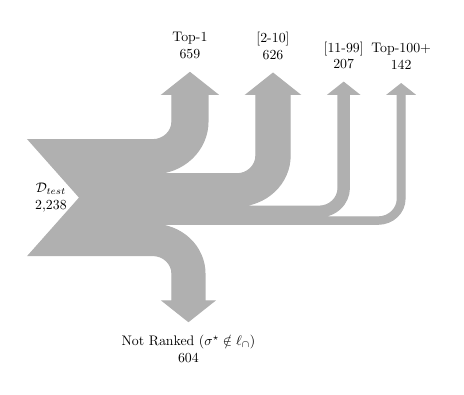
\begin{tikzpicture}

\definecolor{darkgray176}{RGB}{176,176,176}

\begin{axis}[
hide x axis,
hide y axis,
tick align=outside,
tick pos=left,
x grid style={darkgray176},
xmin=-0.65, xmax=2.16685714285714,
xtick style={color=black},
y grid style={darkgray176},
ymin=-1.23407157830616, ymax=1.2406645039797,
ytick style={color=black}
]
\path [draw=darkgray176, fill=darkgray176]
(axis cs:-0.25,0.320142857142857)
--(axis cs:-0.125,0.320142857142857)
.. controls (axis cs:-0.03125,0.320142857142857) and (axis cs:0.03125,0.319714285714286) .. (axis cs:0.125,0.319714285714286)
--(axis cs:0.25,0.319714285714286)
--(axis cs:0.4,0.319714285714286)
.. controls (axis cs:0.4265114773,0.319714285714286) and (axis cs:0.4519642327,0.330257162214286) .. (axis cs:0.4707106781,0.349003607614286)
.. controls (axis cs:0.4894571235,0.367750053014286) and (axis cs:0.5,0.393202808414286) .. (axis cs:0.5,0.419714285714286)
--(axis cs:0.5,0.569714285714286)
--(axis cs:0.45,0.569714285714286)
--(axis cs:0.594142857142857,0.690664503979697)
--(axis cs:0.738285714285714,0.569714285714286)
--(axis cs:0.688285714285714,0.569714285714286)
--(axis cs:0.688285714285714,0.419714285714286)
.. controls (axis cs:0.688285714285714,0.343285484012286) and (axis cs:0.657892107461429,0.269908826302) .. (axis cs:0.603848783436857,0.215865502277429)
.. controls (axis cs:0.549805459412286,0.161822178252857) and (axis cs:0.476428801702,0.131428571428572) .. (axis cs:0.4,0.131428571428572)
--(axis cs:0.688285714285714,0.131428571428571)
--(axis cs:0.838285714285714,0.131428571428571)
.. controls (axis cs:0.864797191585714,0.131428571428571) and (axis cs:0.890249946985714,0.141971447928571) .. (axis cs:0.908996392385714,0.160717893328571)
.. controls (axis cs:0.927742837785714,0.179464338728571) and (axis cs:0.938285714285714,0.204917094128571) .. (axis cs:0.938285714285714,0.231428571428571)
--(axis cs:0.938285714285714,0.569714285714286)
--(axis cs:0.888285714285714,0.569714285714286)
--(axis cs:1.02771428571429,0.686708748575575)
--(axis cs:1.16714285714286,0.569714285714286)
--(axis cs:1.11714285714286,0.569714285714286)
--(axis cs:1.11714285714286,0.231428571428571)
.. controls (axis cs:1.11714285714286,0.157499423300571) and (axis cs:1.08774329296,0.0865225968137143) .. (axis cs:1.03546749093029,0.034246794784)
.. controls (axis cs:0.983191688900572,-0.0180290072457143) and (axis cs:0.912214862413714,-0.0474285714285714) .. (axis cs:0.838285714285714,-0.0474285714285714)
--(axis cs:1.11714285714286,-0.0474285714285714)
--(axis cs:1.26714285714286,-0.0474285714285714)
.. controls (axis cs:1.29365433444286,-0.0474285714285714) and (axis cs:1.31910708984286,-0.0368856949285714) .. (axis cs:1.33785353524286,-0.0181392495285714)
.. controls (axis cs:1.35659998064286,0.000607195871428601) and (axis cs:1.36714285714286,0.0260599512714286) .. (axis cs:1.36714285714286,0.0525714285714286)
--(axis cs:1.36714285714286,0.569714285714286)
--(axis cs:1.31714285714286,0.569714285714286)
--(axis cs:1.39671428571429,0.636482642080821)
--(axis cs:1.47628571428571,0.569714285714286)
--(axis cs:1.42628571428571,0.569714285714286)
--(axis cs:1.42628571428571,0.0525714285714286)
.. controls (axis cs:1.42628571428571,0.0103803061254286) and (axis cs:1.40950747939857,-0.0301259360397143) .. (axis cs:1.37967385057629,-0.059959564862)
.. controls (axis cs:1.349840221754,-0.0897931936842857) and (axis cs:1.30933397958886,-0.106571428571429) .. (axis cs:1.26714285714286,-0.106571428571429)
--(axis cs:1.42628571428571,-0.106571428571429)
--(axis cs:1.57628571428571,-0.106571428571429)
.. controls (axis cs:1.60279719158571,-0.106571428571429) and (axis cs:1.62824994698571,-0.0960285520714286) .. (axis cs:1.64699639238571,-0.0772821066714286)
.. controls (axis cs:1.66574283778571,-0.0585356612714285) and (axis cs:1.67628571428571,-0.0330829058714286) .. (axis cs:1.67628571428571,-0.00657142857142855)
--(axis cs:1.67628571428571,0.569714285714286)
--(axis cs:1.62628571428571,0.569714285714286)
--(axis cs:1.69657142857143,0.62869100264846)
--(axis cs:1.76685714285714,0.569714285714286)
--(axis cs:1.71685714285714,0.569714285714286)
--(axis cs:1.71685714285714,-0.00657142857142855)
.. controls (axis cs:1.71685714285714,-0.0438389909474286) and (axis cs:1.70203687074857,-0.079618292824) .. (axis cs:1.67568472464343,-0.105970438929143)
.. controls (axis cs:1.64933257853829,-0.132322585034286) and (axis cs:1.61355327666171,-0.147142857142857) .. (axis cs:1.57628571428571,-0.147142857142857)
--(axis cs:0.4,-0.147142857142857)
.. controls (axis cs:0.472262712412,-0.147142857142857) and (axis cs:0.541639651416571,-0.175879726231429) .. (axis cs:0.592737105449714,-0.226977180264572)
.. controls (axis cs:0.643834559482857,-0.278074634297714) and (axis cs:0.672571428571429,-0.347451573302286) .. (axis cs:0.672571428571429,-0.419714285714286)
--(axis cs:0.672571428571429,-0.569714285714286)
--(axis cs:0.722571428571429,-0.569714285714286)
--(axis cs:0.586285714285714,-0.684071578306161)
--(axis cs:0.45,-0.569714285714286)
--(axis cs:0.5,-0.569714285714286)
--(axis cs:0.5,-0.419714285714286)
.. controls (axis cs:0.5,-0.393202808414286) and (axis cs:0.4894571235,-0.367750053014286) .. (axis cs:0.4707106781,-0.349003607614286)
.. controls (axis cs:0.4519642327,-0.330257162214286) and (axis cs:0.4265114773,-0.319714285714286) .. (axis cs:0.4,-0.319714285714286)
--(axis cs:0.25,-0.319714285714286)
--(axis cs:0.25,-0.319714285714286)
--(axis cs:0.125,-0.319714285714286)
.. controls (axis cs:0.03125,-0.319714285714286) and (axis cs:-0.03125,-0.320142857142857) .. (axis cs:-0.125,-0.320142857142857)
--(axis cs:-0.25,-0.320142857142857)
--(axis cs:-0.25,-0.320142857142857)
--(axis cs:0.0186317533526121,0)
--(axis cs:-0.25,0.320142857142857)
--(axis cs:0,0.320142857142857)
--(axis cs:-0.25,0.320142857142857)
--cycle;
\draw (axis cs:-0.131368246647388,0) node[
  scale=0.5,
  text=black,
  rotate=0.0,
  align=center
]{$\mathcal{D}_{\text{test}}$\\2,238};
\draw (axis cs:0.594142857142857,0.840664503979697) node[
  scale=0.5,
  text=black,
  rotate=0.0,
  align=center
]{Top-1\\659};
\draw (axis cs:1.02771428571429,0.836708748575575) node[
  scale=0.5,
  text=black,
  rotate=0.0,
  align=center
]{[2-10]\\626};
\draw (axis cs:1.39671428571429,0.786482642080821) node[
  scale=0.5,
  text=black,
  rotate=0.0,
  align=center
]{[11-99]\\207};
\draw (axis cs:1.69657142857143,0.77869100264846) node[
  scale=0.5,
  text=black,
  rotate=0.0,
  align=center
]{Top-100+\\142};
\draw (axis cs:0.586285714285714,-0.834071578306161) node[
  scale=0.5,
  text=black,
  rotate=0.0,
  align=center
]{Not Ranked $(\sigma^\star \notin \ell_\cap)$\\604};
\end{axis}

\end{tikzpicture}
}\end{center}
\vspace{-1.1cm}
\caption{Outcomes in the repair pipeline.}
\label{fig:sankey}
\end{wrapfigure}

\noindent We present a Sankey diagram of the Tidyparse repair pipeline in Fig.~\ref{fig:sankey}. Across 2,238 test set repairs filtered by length and distance ($\lfloor|\err\sigma| / 10\rfloor \in [0, 8], \Delta(\err\sigma, \sigma') < 4$), we evaluated Tidyparse with a timeout of 10s and tracked individual repair outcomes. In 607 cases, the true repair was not contained in the language intersection and thus never sampled, in 1,631 cases the true repair was sampled, of which 675 cases the first prediction matched the true repair, in 1,242 cases, the true repair was in the top-10 results, and in the remaining 389 cases the true repair was drawn, but ranked lower than 10\textsuperscript{th} in the final results.

\clearpage\subsection{Internal evaluation}\label{sec:rq3}

The primary question of interest here is, to what extent does the neural reranker improve precision relative to a na\"ive decoding strategy? For comparison, we use an 4-gram based repair sans reranking. That is, we decode the language intersection with a 4-gram model, sort the repairs by their respective 4-gram probabilities, and without further processing, evaluate Precision@$10^{\{0, 1, 2, 3\}}$.\vspace{-0.2cm}
\begin{figure}[H]
\resizebox{.24\textwidth}{!}{\input{len_dist_ngram_p1}}
\resizebox{.24\textwidth}{!}{\input{len_dist_ngram_p10}}
\resizebox{.24\textwidth}{!}{\input{len_dist_ngram_p100}}
\resizebox{.24\textwidth}{!}{\input{len_dist_ngram_p1000}}
\caption{4-gram repairs. 4-gram Precision@1000 is an upper bound on Tidyparse Precision@k, since the latter only reranks the top-$10^3$ most probable 4-gram sampled repairs from the language intersection.}\label{fig:adaptive}
\end{figure}\vspace{-0.2cm}

\begin{wrapfigure}{r}{0.45\textwidth}
\vspace{-0.35cm}
%\input{experiments/ablation_enumeration_pcfg}
%\input{experiments/ablation_enumeration_markov}
\resizebox{.45\textwidth}{!}{\input{experiments/rank_cdf}}
\vspace{-0.8cm}
\caption{Observed improvement in repair rank with and without the transformer reranker.}
\label{fig:rank_cdf}
\vspace{-0.3cm}
\end{wrapfigure}

We can quantify the ranking improvement by comparing CDFs of the true repair's rank across the test set of human repairs, before and after reranking the top-$10^3$ sampled repairs (Fig.~\ref{fig:rank_cdf}). Since we decode but do not consider less probable repairs, reranking does not affect repairs originally ranked lower. Repairs initially ranked in the top-$10^3$ results by 4-gram probability tend to place between 1\textsuperscript{st} and 10\textsuperscript{th} in about 75\% of instances after reranking. It is possible the true repair can be ranked higher before reranking than after, which occurs in $\sim4\%$ of cases.

Finally, we investigate the impact of increased parallelism on repair throughput. To simulate a realistic editing scenario, we measure the end-to-end wallclock runtime required to construct the Levenshtein automaton, form the intersection regex $(S_\cap)$, decode and rank the entire intersection language $(\ell_\cap)$. Then, we swap in our GPU implementation of the algorithm described in \S~\ref{sec:implementation} as a replacement for the CPU version and compare the individual repair timings across the same test set.
\begin{wrapfigure}{l}{0.38\textwidth}
\vspace{-0.2cm}
\resizebox{.38\textwidth}{!}{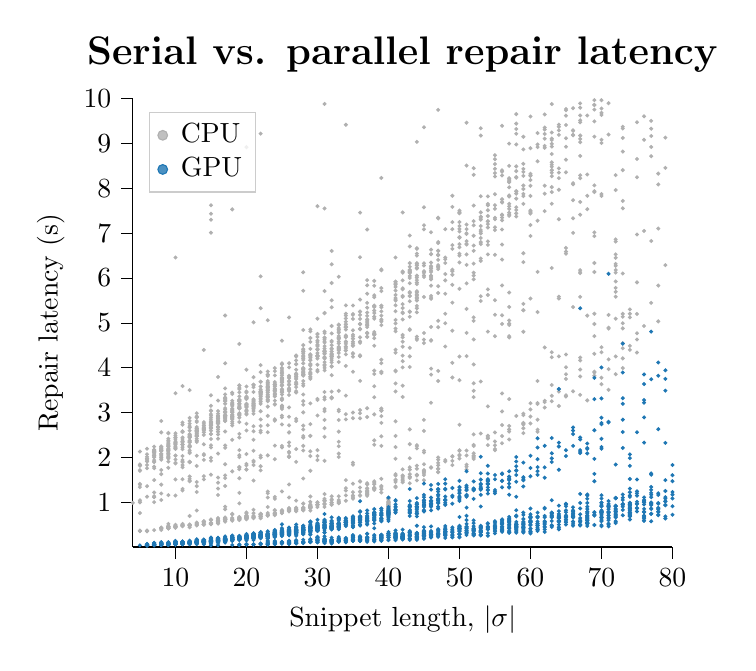
\begin{tikzpicture}
\definecolor{darkgray176}{RGB}{176,176,176}
\definecolor{darkorange25512714}{RGB}{255,127,14}
\definecolor{forestgreen4416044}{RGB}{44,160,44}
\definecolor{lightgray204}{RGB}{204,204,204}
\definecolor{steelblue31119180}{RGB}{31,119,180}
\begin{axis}[
  legend cell align={left},
  legend style={at={(0.85,0.88)}, fill opacity=0.8, draw opacity=1, text opacity=1, draw=lightgray204, legend columns=1, legend pos=north west},
  legend image post style={scale=3.5},
  tick align=outside,
  tick pos=left,
  x grid style={darkdarkgray176},
  xlabel={Snippet length, $|\err\sigma|$},
  xmin=0, xmax=80,
  title={{\Large\textbf{Serial vs. parallel repair latency}}},
  xtick style={color=black},
  y grid style={darkdarkgray176},
  axis lines*=left,
  ylabel={Repair latency (s)},
  ymin=0, ymax=10000,
  xmin=4,
  mark size=0.5pt,
  ytick style={color=black},
  xtick={10, 20, 30, 40, 50, 60, 70, 80},
  ytick={1000,2000,3000,4000,5000,6000,7000,8000,9000,10000},
  scaled y ticks=false,
  yticklabels={
    \(\displaystyle {1}\),
    \(\displaystyle {2}\),
    \(\displaystyle {3}\),
    \(\displaystyle {4}\),
    \(\displaystyle {5}\),
    \(\displaystyle {6}\),
    \(\displaystyle {7}\),
    \(\displaystyle {8}\),
    \(\displaystyle {9}\),
    \(\displaystyle {10}\),
  },
]
\addlegendentry{\phantom{.}CPU}
\addlegendentry{\phantom{.}GPU}
\addplot [draw=darkgray176, fill=darkgray176, mark=*, only marks]
table{
  15	7623
  16	572
  20	771
  75	5199
  51	4777
  71	3507
  34	1032
  31	892
  50	1972
  29	920
  15	509
  29	892
  43	1981
  50	2058
  11	481
  9	442
  24	749
  30	949
  23	893
  25	820
  37	1255
  54	2482
  26	794
  42	1474
  31	948
  44	1814
  70	9085
  20	685
  45	1650
  40	766
  56	2475
  8	419
  38	1402
  33	1004
  75	4768
  41	3918
  11	515
  25	791
  8	423
  29	899
  19	640
  30	995
  77	6826
  27	1034
  26	869
  23	1105
  21	662
  52	2011
  14	502
  36	1153
  30	935
  21	680
  35	1150
  19	602
  59	2729
  31	1076
  73	4208
  27	818
  70	3633
  37	1164
  14	512
  28	825
  78	5831
  29	862
  20	700
  43	1422
  57	2701
  37	1313
  24	1075
  69	4974
  67	3805
  9	433
  30	941
  56	2720
  5	365
  10	463
  17	573
  43	1728
  73	3991
  20	664
  61	2619
  40	738
  19	653
  62	3232
  52	7269
  56	8404
  68	10243
  22	3028
  54	7651
  39	3051
  79	8457
  70	7872
  12	3499
  76	9084
  39	6193
  56	9395
  21	3458
  33	4855
  11	1296
  17	3267
  60	9603
  17	3404
  8	2193
  34	5161
  22	2039
  26	2905
  52	8449
  13	2914
  39	8232
  28	4503
  55	8740
  22	3683
  16	2911
  73	27637
  69	10478
  26	3818
  44	6210
  38	2958
  59	9151
  57	8227
  8	2211
  34	4573
  20	3470
  72	8296
  26	4007
  16	1549
  47	3703
  57	8998
  29	4810
  33	4668
  15	1924
  21	3788
  20	8919
  28	4359
  78	8329
  69	10045
  30	4500
  21	1899
  34	5026
  69	9153
  38	3858
  7	2136
  73	10678
  62	13803
  11	2338
  27	3748
  38	4738
  78	15107
  24	3829
  50	7038
  25	3896
  9	2380
  78	12391
  24	3625
  22	3453
  73	8407
  58	9444
  67	9474
  13	2891
  23	3619
  56	7399
  44	6318
  54	7620
  11	3590
  57	8181
  35	5178
  44	5952
  63	4234
  45	6152
  66	10137
  11	2565
  69	6134
  13	2544
  31	4203
  22	3353
  48	4991
  33	2007
  25	3722
  19	3105
  32	4575
  45	6145
  25	4097
  21	3295
  15	2790
  49	6735
  50	3722
  41	5919
  58	7373
  44	5571
  21	3181
  23	3839
  12	2508
  37	7081
  19	1780
  12	2094
  24	1959
  35	4323
  44	6222
  13	2608
  44	5865
  25	3606
  17	5164
  55	8264
  24	3992
  23	3497
  22	3317
  38	5135
  32	4290
  43	6332
  33	4947
  20	1821
  60	7456
  26	2333
  39	5161
  25	3463
  31	4771
  17	2997
  76	18972
  20	3175
  19	1785
  26	3629
  18	3263
  14	2648
  25	3996
  65	12289
  32	4417
  41	5850
  38	5273
  8	2236
  10	2036
  23	3390
  21	3130
  52	6725
  10	2245
  67	10402
  21	2393
  41	5514
  71	5177
  54	6817
  67	9174
  7	2119
  63	9109
  17	2899
  65	12273
  53	9177
  35	4701
  31	5221
  35	4501
  53	7070
  62	8905
  63	9880
  58	7883
  44	5499
  57	8209
  31	4665
  74	24003
  47	6521
  9	2097
  17	2998
  53	7317
  67	9518
  46	5999
  42	5215
  18	2883
  17	2937
  63	4345
  74	16245
  15	2882
  16	2767
  34	4913
  9	2245
  40	897
  25	3450
  19	1534
  69	25710
  15	7434
  58	8252
  36	4257
  41	2478
  39	3036
  77	12206
  13	2471
  41	6458
  61	11447
  16	3267
  22	3580
  54	7821
  17	3019
  13	2578
  24	3490
  52	15182
  67	6176
  75	14767
  17	3337
  47	7347
  17	3313
  38	5359
  43	6115
  38	5937
  47	5818
  71	10803
  70	10186
  41	4873
  13	2635
  51	6765
  75	8247
  32	5503
  41	5866
  42	5417
  73	11209
  19	3289
  57	5054
  60	8056
  16	2571
  22	3416
  38	4797
  69	9858
  30	3915
  41	5720
  34	4680
  60	7508
  34	4296
  12	2355
  39	5346
  28	3846
  6	1830
  19	2965
  59	8433
  28	3704
  23	10399
  65	4295
  30	4265
  40	924
  47	6287
  52	6321
  71	11541
  29	4085
  38	4657
  9	2165
  73	11646
  26	1396
  11	2361
  15	2595
  20	3043
  14	1579
  56	7684
  13	2344
  18	2925
  41	5391
  16	2416
  29	4167
  65	18701
  40	783
  60	8323
  73	10793
  34	3377
  28	3823
  11	2283
  49	17006
  76	11631
  12	2597
  9	2165
  16	2881
  7	1939
  36	7459
  34	4474
  41	4811
  9	2205
  24	3358
  36	2871
  24	3463
  12	2231
  69	9758
  23	3561
  71	10127
  25	3111
  50	13297
  31	4355
  8	2161
  14	2785
  50	6544
  33	4782
  8	2155
  35	4487
  45	6115
  24	2261
  46	3845
  34	1491
  56	10605
  52	4072
  74	10118
  41	2230
  71	10194
  20	3026
  29	1701
  78	13063
  56	7417
  7	1758
  57	7600
  69	10055
  65	10013
  57	8157
  17	2938
  73	11719
  42	5771
  18	2953
  21	3034
  49	6187
  70	9781
  36	4868
  71	11710
  18	2709
  47	5666
  43	4252
  23	3132
  22	3282
  54	6738
  45	6278
  46	5557
  20	2073
  63	8482
  24	3186
  9	2088
  52	6118
  15	2518
  31	3940
  25	3282
  12	2473
  32	4214
  60	7480
  35	2874
  65	8357
  41	5553
  37	4781
  18	2754
  63	8348
  15	2521
  42	4468
  77	12061
  70	13497
  24	3632
  75	23255
  17	2577
  35	4309
  73	11275
  33	2573
  51	6823
  48	6456
  68	9626
  51	8508
  69	10474
  38	5384
  24	3680
  23	3915
  17	3196
  11	2444
  21	3271
  26	2008
  58	8384
  27	3955
  70	12661
  18	3412
  50	6348
  23	10599
  77	12601
  72	6862
  30	4067
  43	6253
  19	3281
  23	5057
  29	4577
  10	3430
  47	3927
  51	6747
  17	2826
  33	4817
  50	6903
  44	6649
  8	2812
  70	12547
  22	4056
  23	1239
  76	14233
  20	3956
  6	1358
  59	8868
  49	7089
  13	1358
  53	9340
  26	2100
  40	873
  56	7082
  19	3449
  44	6277
  77	22576
  75	11000
  25	3760
  31	3080
  8	2244
  58	7939
  13	2787
  12	2518
  44	15758
  73	7720
  32	4312
  13	1451
  48	4474
  38	5372
  14	2703
  58	8240
  23	3504
  24	2849
  13	2541
  76	12423
  19	3523
  56	7288
  67	10314
  50	6916
  73	6101
  7	2155
  70	10932
  8	2144
  53	3692
  79	9131
  25	3783
  22	3448
  15	2713
  42	5747
  25	3402
  22	3902
  41	3470
  56	7699
  25	3615
  55	4703
  67	9626
  28	3961
  37	5338
  16	2761
  72	6315
  34	4384
  69	7917
  31	4427
  6	1975
  30	4571
  29	4299
  33	4406
  17	2917
  35	4245
  24	3421
  48	6336
  59	8277
  18	3089
  23	2044
  12	2377
  39	5028
  71	10186
  53	7825
  26	2714
  62	9312
  10	2407
  30	4257
  8	2080
  25	3752
  28	4096
  73	9374
  8	1049
  45	6022
  18	3197
  34	5204
  63	8406
  67	9895
  36	5519
  14	2746
  55	7543
  15	2755
  21	3197
  37	4764
  73	7554
  23	3409
  46	6533
  56	8371
  26	2557
  13	2476
  17	2882
  40	863
  34	4902
  58	9325
  63	8527
  53	6434
  70	7830
  51	6982
  53	12170
  19	3091
  9	1992
  31	4325
  77	11415
  46	15793
  56	8288
  61	9233
  57	7422
  38	5353
  35	4580
  37	4906
  45	2836
  56	7757
  58	9219
  28	6127
  68	11036
  31	4559
  68	10328
  27	3872
  26	3543
  42	4144
  37	4692
  48	6088
  13	2036
  68	8308
  20	1726
  57	4702
  17	1361
  31	1923
  38	2379
  62	7881
  27	3839
  27	3773
  47	6612
  11	2568
  26	3793
  67	7697
  71	11398
  17	2809
  50	7458
  50	12949
  6	1920
  34	4439
  57	8024
  42	7463
  17	2265
  30	1940
  28	3174
  27	3625
  7	2135
  13	2599
  25	3080
  23	3846
  20	3183
  55	7342
  38	5138
  9	2535
  15	2770
  22	3464
  24	3392
  32	4119
  30	3280
  70	10234
  31	3030
  37	3095
  73	10917
  78	11050
  30	4415
  19	3599
  57	7541
  13	2810
  25	3130
  76	12916
  8	2184
  55	6518
  50	7161
  52	7616
  46	5537
  50	4248
  43	6949
  19	3262
  69	12840
  18	3181
  22	3515
  54	5622
  46	6345
  61	11393
  71	9899
  69	11332
  34	4972
  6	2013
  24	3626
  26	2011
  19	2524
  68	7536
  14	2663
  32	4930
  36	11706
  68	10675
  45	7178
  38	4488
  77	24386
  20	2599
  27	1899
  6	1123
  39	5061
  46	6173
  49	5849
  6	1958
  39	2256
  38	5574
  58	9656
  59	6356
  13	1228
  51	5311
  14	1944
  12	2466
  16	2512
  31	4044
  44	4647
  31	4383
  7	1002
  23	3570
  16	2577
  46	5600
  23	3589
  28	4398
  33	4584
  40	982
  24	3923
  14	2602
  60	7181
  37	5156
  30	4517
  58	7442
  74	11281
  5	1820
  57	7817
  43	4841
  36	2984
  45	6058
  13	2593
  56	4976
  15	7011
  70	10607
  39	2768
  43	5606
  59	7654
  34	4959
  15	2270
  7	1134
  18	3009
  24	3266
  56	5834
  31	7552
  25	2254
  29	3965
  52	6055
  47	6253
  23	3544
  44	5553
  33	4126
  66	10318
  49	7835
  36	14151
  42	6147
  73	9335
  40	858
  17	2941
  29	3873
  25	3518
  29	3203
  39	5079
  15	3149
  31	4671
  37	5954
  39	6172
  17	2852
  49	7586
  34	4530
  21	3213
  15	2221
  25	3739
  34	4588
  8	1626
  30	4409
  22	1710
  31	3996
  32	3467
  16	3032
  63	8272
  14	2708
  23	1198
  52	3343
  31	3343
  28	3891
  45	2590
  16	2084
  78	14078
  32	6306
  42	5602
  7	1494
  75	10616
  71	10117
  23	3361
  71	9200
  43	6120
  21	2973
  11	1261
  43	5592
  64	9374
  30	3947
  20	3114
  12	2249
  29	4662
  38	3934
  34	5390
  44	6545
  8	2075
  15	2964
  34	4690
  16	3794
  20	3147
  6	1905
  73	22300
  34	4848
  65	8929
  15	2717
  51	6293
  43	6150
  15	2836
  10	2201
  53	11291
  19	3168
  30	4401
  54	7201
  40	945
  19	3361
  39	4949
  73	12011
  44	6333
  53	18102
  8	2029
  55	7625
  12	2340
  36	5254
  40	958
  74	11104
  33	2084
  9	2009
  63	10582
  15	2642
  41	5917
  63	9078
  16	2803
  61	7278
  10	2041
  50	7247
  46	5969
  63	9246
  79	13025
  36	4855
  16	2664
  21	3079
  32	3334
  79	13036
  19	3117
  53	6382
  19	2931
  28	10701
  75	16643
  31	5708
  31	4307
  34	9419
  10	1148
  43	4015
  39	4178
  5	1713
  30	4752
  58	7771
  48	5203
  32	4430
  46	4909
  6	2069
  64	4253
  26	3768
  15	2409
  11	1900
  59	5285
  40	1080
  53	7464
  20	3334
  14	2632
  48	7090
  35	5387
  31	4361
  21	3097
  59	4801
  23	3703
  33	4884
  50	7470
  22	3687
  25	2892
  45	9363
  49	7248
  11	2730
  40	712
  16	2858
  55	7069
  44	2199
  32	4597
  12	2813
  45	7577
  43	5137
  10	2538
  38	5826
  29	4854
  21	3619
  50	7443
  71	11143
  54	6526
  19	3547
  20	3340
  43	6174
  17	3019
  33	4327
  72	5693
  32	6604
  10	2490
  19	974
  49	6649
  16	1160
  18	3443
  28	3993
  45	4548
  44	4621
  54	7512
  14	2560
  56	10480
  5	1041
  19	3132
  33	2247
  11	1941
  51	9465
  47	6243
  47	6604
  41	4988
  42	5076
  23	3250
  18	2879
  28	3977
  43	4443
  23	2925
  21	3612
  23	3816
  32	4254
  44	5534
  60	6937
  35	4833
  35	5195
  29	4048
  36	3706
  39	3046
  13	2364
  47	5046
  46	6056
  52	6943
  63	8404
  77	9330
  23	3332
  45	5578
  24	2817
  30	4244
  17	2814
  56	7348
  19	3197
  27	3654
  23	2715
  42	5947
  34	4901
  18	3219
  16	2799
  36	4555
  11	2581
  9	2061
  58	12404
  41	2803
  36	5087
  31	4220
  62	8059
  18	3031
  57	4984
  22	2845
  20	3580
  9	2253
  12	2481
  8	2051
  13	2516
  31	4636
  8	2557
  28	4216
  50	6755
  61	8980
  33	4961
  5	758
  57	7457
  50	2727
  25	3600
  44	9038
  43	2295
  13	2377
  67	10520
  5	1700
  35	4645
  10	2279
  62	10287
  16	2772
  36	4980
  36	4586
  52	8302
  31	4481
  28	4250
  20	3146
  9	2418
  66	9196
  10	2438
  12	2881
  22	3403
  20	3056
  35	3909
  9	2142
  27	3805
  49	4825
  7	1892
  23	3287
  22	2596
  66	9295
  28	3597
  7	1114
  19	3252
  13	2416
  20	2984
  26	5121
  46	6214
  33	4465
  9	2029
  43	5245
  37	4965
  17	1598
  20	2957
  71	18660
  56	7752
  59	7878
  27	3679
  9	2188
  16	2622
  42	4268
  46	4602
  31	4362
  11	2180
  27	4246
  57	3300
  31	4324
  66	10075
  49	15029
  61	8920
  43	5685
  71	10485
  73	13881
  47	6200
  12	1521
  36	4678
  57	12043
  33	4239
  12	2157
  64	8352
  27	3478
  42	3347
  32	3337
  34	2962
  19	3257
  28	3986
  38	3339
  16	2798
  37	4998
  60	8185
  58	7518
  45	2148
  57	4954
  15	2726
  45	4774
  46	6532
  30	4272
  27	2810
  37	5041
  15	2928
  20	3316
  49	14947
  20	3300
  40	878
  11	2357
  13	2489
  29	4222
  9	1158
  23	3458
  56	3425
  78	14920
  33	4666
  33	4431
  68	11478
  72	6272
  60	7437
  31	4589
  55	8436
  22	5327
  41	5623
  5	1336
  30	4480
  70	13515
  10	2359
  31	3458
  73	10974
  77	12705
  48	12174
  18	1687
  35	10663
  53	7299
  17	3064
  25	3156
  28	1528
  43	6705
  36	5176
  30	7603
  75	6972
  12	2442
  51	7091
  35	4733
  17	1537
  31	3293
  10	2447
  49	3781
  19	3204
  19	2986
  72	6179
  11	1778
  53	7365
  35	5088
  78	12299
  7	1114
  64	9423
  15	3046
  7	2239
  28	4840
  75	11949
  13	2984
  12	2666
  26	4101
  15	3036
  42	6119
  49	5450
  6	2191
  76	14357
  10	2325
  26	3391
  40	848
  29	10455
  36	4967
  29	3803
  23	3656
  13	2574
  47	4903
  17	3538
  29	4269
  77	9505
  22	3371
  9	2281
  18	2918
  10	1952
  24	3516
  16	2862
  13	816
  35	4653
  59	7986
  59	6553
  27	4081
  15	2721
  69	26225
  23	3498
  44	6664
  44	5675
  57	8133
  23	3668
  29	4258
  72	6813
  62	7492
  63	8993
  42	5331
  5	1409
  31	5216
  52	7176
  27	4272
  40	670
  69	9864
  75	8656
  31	2457
  18	2794
  38	2281
  21	3158
  69	7936
  18	3003
  37	4685
  11	1894
  44	2274
  43	5482
  26	3519
  66	8090
  7	2172
  67	10815
  17	3098
  11	2228
  12	2447
  48	5947
  53	6801
  28	4279
  59	7827
  42	3598
  32	4243
  27	2858
  75	11058
  40	966
  45	4626
  15	1614
  26	2024
  4	986
  20	1731
  21	1828
  67	6110
  69	10208
  64	18970
  70	10427
  26	2123
  14	2071
  33	6027
  18	2900
  25	4603
  54	7269
  26	3507
  12	1466
  56	6747
  20	1853
  60	8279
  21	3247
  35	4496
  30	5094
  37	5230
  31	4124
  12	2268
  36	5249
  16	1436
  22	3426
  21	2693
  5	1813
  18	2845
  12	1895
  46	6267
  41	5259
  47	6506
  44	5326
  76	12256
  8	1392
  19	2787
  5	1000
  18	2915
  29	3774
  30	3303
  37	5445
  8	1962
  10	2296
  23	3586
  29	4170
  40	999
  75	11093
  38	4765
  71	11300
  20	3142
  77	8923
  43	6047
  40	1001
  69	6936
  64	19154
  38	5093
  64	8447
  26	3706
  18	2391
  29	4285
  13	1809
  51	6999
  65	9743
  52	10235
  6	1756
  12	2334
  11	2030
  64	5543
  44	5380
  22	1802
  51	5881
  17	899
  14	2049
  56	5169
  29	2742
  9	1904
  66	9283
  73	11649
  30	4203
  61	8604
  66	7736
  75	12122
  45	2108
  41	5886
  62	9108
  28	3846
  33	2348
  43	5669
  39	5777
  53	7363
  70	11034
  43	5255
  59	8548
  23	3445
  38	5616
  18	3050
  48	6420
  18	2873
  7	2041
  21	5011
  44	6289
  62	8948
  78	11729
  8	2140
  40	1085
  25	3518
  54	7127
  57	7843
  55	8340
  43	6154
  32	4361
  33	4445
  9	1767
  15	2719
  40	1014
  46	7021
  44	5900
  15	2777
  17	4098
  49	4109
  55	7131
  7	2111
  37	4942
  53	6757
  40	1005
  13	2646
  19	2442
  25	3671
  16	2758
  69	8068
  24	3540
  63	8028
  20	2750
  25	3700
  38	5218
  39	5256
  19	2162
  47	9751
  44	6226
  8	1946
  25	3928
  37	5072
  66	10345
  69	9969
  30	4749
  66	18306
  41	5801
  5	2130
  25	3867
  28	2256
  13	2889
  11	2778
  28	4359
  29	3853
  28	3003
  55	8651
  7	2160
  14	2500
  40	940
  21	3211
  46	6248
  11	2293
  63	7917
  25	4075
  43	4859
  71	13717
  27	3808
  25	3829
  32	4255
  25	3484
  79	12508
  33	4642
  28	3255
  19	3089
  58	13244
  47	6405
  51	7192
  23	3504
  35	2998
  30	4263
  76	12074
  13	2473
  39	4100
  40	813
  75	10775
  44	6007
  63	8932
  17	2938
  76	10695
  21	3159
  37	5080
  35	4543
  14	2291
  15	2674
  7	2098
  15	2669
  33	4542
  17	2874
  16	2752
  66	8115
  24	3590
  70	9684
  62	9214
  19	4530
  50	6685
  75	13186
  8	1999
  72	5780
  66	5352
  12	2752
  28	3915
  57	5354
  65	9414
  29	3897
  5	1389
  25	3602
  79	12920
  65	6672
  31	9883
  69	7018
  57	8501
  36	4973
  71	10639
  67	11742
  19	2969
  45	6327
  16	2934
  33	4385
  63	6223
  45	7086
  7	2030
  65	11880
  67	9030
  23	3358
  5	1843
  27	3567
  32	3316
  75	12886
  41	3648
  26	3686
  21	2581
  43	5884
  57	7655
  9	2547
  34	4720
  49	6073
  28	3948
  38	4737
  64	8230
  53	7159
  41	5066
  35	1881
  60	7832
  10	2306
  19	2885
  36	4278
  27	2185
  58	7579
  57	7388
  55	7310
  77	9168
  42	4006
  26	3113
  6	1976
  31	2834
  10	1878
  58	10595
  19	3608
  72	5093
  29	4073
  65	9622
  40	785
  27	4075
  27	3847
  7	1217
  58	7928
  44	6500
  24	3589
  12	1892
  21	3563
  44	5637
  12	2115
  9	1971
  63	8580
  49	6156
  72	7963
  10	1863
  53	6892
  30	4326
  39	5385
  28	2707
  47	6780
  9	2344
  50	7095
  31	4220
  22	2558
  7	1998
  65	9118
  19	1736
  32	12824
  39	3091
  64	5584
  65	9769
  60	8289
  27	3447
  28	4323
  18	3063
  18	7531
  65	6589
  66	9789
  62	9356
  47	6803
  39	5378
  55	8541
  41	5496
  25	3668
  10	2215
  49	6153
  52	6607
  51	6527
  79	10361
  73	9125
  31	4238
  28	2153
  22	3466
  36	6464
  69	13647
  15	2793
  13	2675
  66	7333
  33	4706
  42	5582
  12	1902
  63	8767
  20	3196
  38	4734
  21	1482
  58	8490
  31	4068
  39	5708
  70	9967
  28	3845
  34	4384
  16	2821
  32	4502
  28	3643
  13	2476
  10	6458
  28	3403
  28	3879
  40	900
  26	3478
  32	4024
  73	8820
  44	4691
  14	2626
  52	5044
  22	3240
  40	752
  28	5716
  46	6633
  10	2187
  20	3446
  55	7870
  16	2776
  53	5489
  53	6995
  64	9194
  66	9184
  7	1793
  7	1905
  15	1989
  62	9648
  7	2073
  70	9013
  32	4168
  50	6900
  16	2688
  30	2030
  9	2143
  64	9295
  52	3652
  53	7032
  43	6184
  64	11656
  28	4170
  29	4419
  22	3479
  50	7506
  44	5705
  76	11606
  9	2312
  42	5233
  25	2734
  59	8368
  32	4763
  44	6054
  15	7300
  22	3194
  11	2285
  71	10210
  30	4687
  69	10721
  37	5838
  21	3121
  52	5122
  41	4401
  54	7262
  59	8064
  40	934
  29	3751
  58	10897
  8	1718
  32	4033
  39	3882
  69	9495
  9	2255
  44	5236
  22	6038
  12	2242
  56	6411
  20	3355
  22	9220
  26	3615
  50	16048
  15	3383
  47	7328
  67	9179
  11	2409
  40	1050
  72	6121
  32	3832
  25	2220
  13	2631
  52	3484
  19	2950
  23	3275
  60	10350
  38	3586
  5	998
  59	5281
  42	4580
  53	5593
  14	4396
  20	3318
  16	2975
  70	9636
  50	6500
  32	5889
  14	1508
  68	11629
  34	5098
  28	4206
  67	23713
  46	6135
  22	3457
  52	5972
  54	7383
  28	3987
  65	8640
  63	3613
  60	8897
  28	4416
  72	5923
  27	4162
  40	1094
  10	2336
  32	5347
  67	5580
  40	788
  67	9102
  34	4039
  19	3097
  17	2931
  75	10405
  25	3448
  13	2594
  64	7311
  48	5649
  16	603
  50	2158
  38	1309
  41	1491
  27	797
  20	630
  69	3914
  30	997
  31	1032
  56	2315
  59	2759
  7	376
  14	501
  12	477
  46	1770
  35	1836
  52	2255
  59	2542
  27	848
  44	1486
  9	461
  47	1742
  56	3025
  31	1025
  70	3777
  17	625
  32	1046
  29	950
  19	1207
  12	478
  78	5033
  68	5161
  16	597
  55	2160
  33	1132
  9	416
  39	1522
  19	666
  20	665
  18	724
  64	3145
  73	4877
  40	757
  9	517
  55	2556
  36	1460
  25	813
  69	3821
  14	566
  40	904
  39	1340
  45	1698
  74	10836
  25	810
  71	4871
  31	1181
  45	1717
  69	4703
  41	1625
  45	1671
  11	485
  37	1235
  47	1747
  16	563
  60	2757
  41	1351
  33	1047
  14	567
  40	768
  45	1605
  24	813
  22	741
  57	5677
  17	615
  20	698
  36	1466
  52	2512
  42	1579
  21	755
  25	758
  49	2015
  55	2185
  22	741
  22	669
  76	10826
  20	744
  36	1237
  15	601
  76	7050
  25	785
  77	8717
  26	833
  41	4334
  11	474
  21	641
  61	3211
  39	2470
  62	3262
  57	2573
  20	618
  36	1233
  43	2624
  59	2942
  10	456
  9	458
  17	619
  37	1300
  49	1920
  8	426
  12	492
  60	2909
  10	495
  57	2399
  54	3137
  18	649
  10	444
  12	440
  15	525
  59	2769
  5	361
  22	724
  24	731
  23	710
  26	856
  8	416
  52	1965
  24	1116
  73	5137
  9	417
  30	891
  35	1224
  35	1137
  67	3958
  16	584
  17	590
  11	470
  6	366
  49	2027
  36	1145
  23	707
  27	830
  20	643
  37	1171
  5	357
  38	1296
  74	5204
  40	793
  28	969
  57	2625
  29	1127
  28	846
  37	1231
  12	472
  30	952
  15	612
  38	1466
  26	813
  45	1492
  13	546
  15	540
  14	575
  12	502
  14	508
  20	675
  54	2453
  42	1444
  22	696
  24	762
  48	1908
  25	1240
  36	1328
  16	523
  32	1065
  65	3356
  20	631
  62	3112
  76	11289
  17	658
  29	905
  8	435
  55	2268
  71	4892
  11	463
  55	2355
  65	3384
  22	720
  15	610
  43	1723
  9	456
  28	845
  28	879
  61	2569
  12	692
  59	2976
  26	1106
  38	1298
  17	611
  72	4250
  41	1969
  45	1846
  12	483
  23	759
  68	3271
  65	3749
  29	930
  44	1592
  9	433
  31	969
  53	2533
  59	2649
  38	1327
  57	2619
  24	709
  15	527
  31	959
  29	898
  34	1313
  19	669
  8	383
  10	446
  70	4456
  67	4226
  54	2420
  47	1948
  48	1939
  26	810
  32	993
  9	468
  41	1502
  10	465
  14	564
  43	1571
  31	1047
  68	7833
  24	825
  15	512
  29	883
  17	842
  16	593
  5	355
  34	1152
  51	1791
  72	5584
  69	3889
  29	881
  18	612
  47	1997
  74	5299
  9	416
  41	1451
  39	2920
  65	3854
  21	660
  71	4186
  14	503
  43	1540
  37	1395
  66	3474
  17	614
  64	7969
  37	1405
  23	703
  64	3467
  17	565
  18	627
  15	529
  79	6286
  54	2274
  47	1677
  42	1496
  46	4615
  76	9607
  32	985
  63	3251
  37	1425
  29	879
  43	1559
  45	1694
  52	2277
  43	1778
  6	361
  30	2934
  58	2924
  28	966
  38	1275
  51	1837
  40	830
  35	1077
  61	2840
  13	502
  17	618
  62	4451
  44	1746
  6	354
  47	1743
  34	1260
  54	5747
  20	659
  13	479
  39	1362
  75	4337
  47	1876
  76	10210
  35	1097
  51	1727
  19	641
  38	1315
  38	1407
  10	475
  44	2251
  29	878
  32	943
  29	873
  20	692
  22	681
  43	1625
  74	4397
  16	547
  52	2040
  73	4992
  52	2005
  13	528
  9	452
  22	684
  77	5446
  73	4434
  41	1331
  28	868
  46	3218
  17	638
  39	1289
  28	875
  70	4345
  23	2560
  20	655
  37	1210
  18	587
  73	4543
  47	1823
  22	641
  42	1733
  75	4629
  26	827
  19	609
  19	623
  17	635
  76	30011
  16	648
  27	880
  50	2039
  15	535
  75	5903
  52	2091
  50	2145
  21	672
  18	598
  6	354
  74	4486
  23	699
  20	659
  76	4930
  42	1596
  60	3070
  51	2152
  21	695
  37	1189
  44	1612
  64	3515
  39	1215
  38	1443
  13	494
  22	723
  28	817
  32	1132
  73	5200
  78	8088
  26	807
  37	1140
  14	554
  10	441
  19	625
  27	849
  25	756
  10	458
  47	1667
  26	845
  74	5123
  20	662
  23	732
  59	2748
  28	848
  75	10517
  20	638
  65	4009
  69	5204
  31	1038
  78	7103
  27	831
  67	4162
  60	3206
  32	951
  29	1009
  33	1020
  69	4310
  41	1593
  63	3372
  10	449
  16	529
  51	2043
  49	1828
  33	984
  20	688
  24	737
  35	1413
  11	493
  67	3394
  61	3190
  72	3854
  71	3968
  18	609
  18	739
  29	812
  33	3483
  42	4678
  46	1777
  72	6452
  24	754
  30	949
  33	978
  16	631
  21	831
  9	418
  10	427
  42	1540
  11	496
  10	1508
  36	3055
  61	5240
  17	2213
  46	5830
  63	7657
  69	10223
  24	3490
  18	3149
  60	14823
  50	5759
  12	2698
  30	4604
  33	4656
  67	8227
  67	9799
  75	9474
  49	10039
  17	3297
  43	5999
  67	8292
  58	8980
  21	3619
  25	3972
  61	3703
  25	2930
  67	8722
  41	3935
  25	3284
  46	6027
  65	6544
  31	4806
  44	6048
  24	3176
  67	10496
  24	3400
  69	10883
  22	2700
  25	3317
  37	5650
  17	3251
  36	4262
  11	1827
  55	5180
  28	2478
  61	6137
  19	2004
  33	3062
  21	2147
  72	6527
  51	4258
  29	2477
  8	1195
  42	4729
  57	4675
  33	2834
  37	2900
  16	1304
  29	2478
  29	2135
  31	2650
  78	30005
  59	5424
  69	6335
  39	3909
  12	1482
  52	4629
  67	6131
  33	3030
  26	2256
  32	4283
  55	5506
  60	5542
  28	2440
  29	2029
  67	7412
  34	2846
  22	1996
  21	1922
  61	13593
  54	4804
  44	5606
  11	1512
  28	2621
  66	7007
  26	2556
  30	2161
  12	1574
  19	2048
  17	1846
  46	3979
};

\addplot [draw=steelblue31119180, fill=steelblue31119180, mark=*, only marks]
table{
    71 844
    14 111
    24 132
    59 490
    28 402
    7 64
    26 380
    10 122
    70 670
    42 210
    64 589
    15 164
    54 393
    35 176
    29 562
    13 108
    56 340
    64 500
    14 157
    75 2560
    73 2841
    35 479
    10 85
    52 417
    64 3525
    13 113
    70 772
    11 102
    33 653
    62 441
    57 1571
    12 110
    23 63
    29 438
    47 243
    58 378
    6 42
    31 323
    38 768
    36 661
    46 460
    64 713
    53 1409
    21 297
    79 1250
    58 421
    44 750
    24 275
    42 262
    65 709
    30 411
    45 321
    10 65
    64 657
    31 126
    68 1173
    22 80
    17 238
    47 867
    21 213
    52 1263
    25 104
    65 947
    21 279
    77 934
    77 972
    16 180
    49 357
    15 110
    33 621
    25 314
    44 236
    11 91
    37 816
    36 172
    50 287
    14 149
    26 273
    69 1965
    22 254
    38 591
    62 558
    23 196
    42 233
    18 245
    51 1372
    18 175
    11 98
    28 430
    70 573
    10 76
    33 396
    27 310
    45 295
    64 441
    43 935
    55 1512
    34 558
    74 987
    32 78
    58 1801
    54 1512
    51 879
    14 134
    24 331
    39 266
    12 85
    43 340
    16 144
    68 685
    63 703
    25 255
    22 298
    18 176
    31 501
    8 75
    25 286
    45 183
    28 300
    75 1506
    57 1531
    76 791
    33 168
    42 167
    74 1118
    45 276
    12 115
    39 813
    35 259
    25 97
    9 51
    29 328
    19 184
    51 315
    47 977
    34 547
    19 196
    27 290
    70 936
    8 48
    13 98
    30 437
    46 330
    47 988
    16 127
    42 239
    19 183
    57 409
    25 373
    44 283
    70 912
    47 1406
    13 93
    36 146
    30 373
    37 568
    19 219
    23 263
    45 258
    21 253
    57 443
    56 543
    37 644
    13 152
    76 1029
    43 326
    20 200
    36 587
    69 3299
    56 393
    72 1839
    34 587
    71 1025
    25 76
    46 915
    33 493
    16 152
    32 419
    55 1272
    17 195
    11 98
    49 439
    72 672
    33 404
    9 81
    52 258
    36 683
    61 525
    58 426
    21 62
    68 2207
    73 898
    47 1035
    24 318
    49 281
    58 383
    28 435
    44 174
    54 1412
    32 523
    11 89
    16 138
    42 179
    8 68
    8 73
    19 153
    45 993
    53 1164
    57 1500
    39 636
    47 901
    55 351
    35 226
    61 476
    29 366
    23 245
    46 978
    70 625
    48 344
    22 71
    28 103
    15 38
    22 221
    27 89
    20 257
    47 1141
    74 853
    36 146
    17 147
    40 849
    33 153
    28 88
    41 808
    22 229
    60 576
    22 227
    33 191
    41 153
    57 1498
    46 277
    49 334
    13 137
    7 63
    46 342
    35 155
    67 730
    29 275
    61 2218
    39 263
    39 745
    26 331
    33 524
    26 292
    48 343
    35 441
    34 489
    31 474
    26 119
    18 185
    74 701
    15 152
    78 1200
    30 442
    23 68
    26 104
    26 329
    45 822
    49 1118
    26 125
    29 353
    8 52
    15 153
    8 45
    39 186
    78 855
    41 950
    14 133
    14 145
    63 1896
    68 592
    36 215
    31 138
    56 397
    39 240
    27 365
    23 222
    26 424
    24 59
    18 257
    59 322
    74 1153
    61 1959
    17 178
    18 163
    46 944
    25 333
    13 170
    29 432
    33 522
    44 182
    27 381
    27 118
    7 83
    23 265
    18 208
    31 151
    61 657
    29 110
    51 375
    21 214
    16 149
    38 600
    30 409
    14 118
    24 248
    57 1689
    28 285
    10 56
    31 470
    40 295
    17 163
    58 460
    28 433
    16 40
    8 93
    65 2029
    31 94
    30 386
    16 153
    38 758
    36 477
    64 392
    80 1169
    41 764
    10 72
    67 2096
    76 949
    29 418
    36 202
    13 131
    43 311
    24 289
    20 199
    31 496
    75 958
    31 736
    21 197
    31 420
    67 860
    15 87
    10 66
    72 1089
    68 643
    26 381
    77 994
    25 327
    76 586
    35 674
    56 371
    68 984
    79 1080
    25 336
    54 1812
    29 569
    35 644
    16 202
    18 169
    22 242
    27 382
    56 520
    18 156
    41 306
    23 268
    37 749
    68 1147
    15 212
    41 243
    53 451
    42 226
    36 793
    13 92
    15 135
    43 239
    12 114
    20 225
    67 2399
    37 293
    22 286
    11 60
    71 780
    51 696
    11 108
    25 507
    19 235
    39 274
    28 116
    28 440
    6 38
    34 144
    79 2322
    38 775
    41 318
    38 614
    15 144
    67 1183
    72 1094
    12 104
    76 998
    76 3849
    30 428
    80 1084
    59 567
    23 299
    40 750
    32 100
    17 168
    72 758
    50 1278
    62 559
    10 83
    74 1810
    36 663
    21 275
    29 174
    55 436
    10 89
    29 438
    36 635
    34 145
    6 40
    54 459
    80 1830
    16 191
    29 126
    70 795
    55 358
    79 1114
    36 170
    23 338
    38 723
    30 205
    76 3635
    22 256
    11 68
    24 133
    12 90
    60 545
    76 2892
    15 147
    48 953
    13 118
    46 213
    33 492
    24 366
    40 827
    26 112
    11 104
    36 219
    31 421
    17 165
    8 84
    29 427
    21 270
    14 134
    8 56
    25 322
    13 162
    51 373
    30 364
    20 185
    70 2230
    26 352
    27 140
    28 394
    72 576
    44 830
    50 414
    65 617
    75 794
    27 364
    10 70
    40 789
    24 313
    50 431
    25 263
    50 1029
    42 232
    49 322
    21 227
    24 270
    9 73
    14 106
    15 144
    30 370
    42 222
    30 449
    58 504
    43 901
    60 405
    32 145
    35 517
    25 77
    22 323
    80 1228
    40 154
    23 261
    20 264
    58 1457
    35 134
    15 131
    11 116
    41 370
    24 342
    29 290
    17 210
    57 632
    10 120
    12 114
    27 434
    54 1331
    7 94
    75 862
    74 706
    20 261
    71 892
    42 294
    20 51
    69 771
    39 646
    47 1027
    74 810
    76 998
    76 632
    26 352
    62 455
    32 451
    39 165
    39 215
    42 242
    23 116
    19 196
    17 131
    34 589
    35 218
    50 1073
    68 900
    45 918
    65 501
    44 282
    36 599
    53 1297
    48 939
    29 441
    20 197
    30 143
    47 308
    30 105
    17 163
    35 550
    50 1477
    22 268
    60 301
    32 145
    10 68
    53 447
    57 560
    68 753
    7 47
    32 468
    53 325
    50 288
    57 501
    78 877
    14 130
    17 172
    23 244
    41 290
    20 197
    70 2739
    23 194
    29 380
    62 336
    35 150
    78 1162
    19 59
    13 111
    19 233
    21 264
    71 460
    44 195
    77 862
    21 259
    68 621
    66 679
    47 857
    15 126
    34 553
    52 399
    22 247
    20 196
    26 101
    20 58
    59 519
    59 1541
    54 251
    42 243
    58 683
    13 134
    15 129
    74 941
    12 60
    36 646
    53 356
    9 81
    61 399
    40 721
    16 162
    73 1101
    6 69
    21 305
    36 662
    30 453
    14 130
    29 485
    57 1568
    21 273
    33 526
    53 260
    36 136
    43 357
    30 359
    15 105
    45 1048
    35 555
    27 79
    37 222
    46 1013
    52 272
    61 2424
    22 240
    35 648
    17 172
    11 61
    35 224
    77 1208
    34 203
    41 230
    65 579
    32 455
    63 484
    24 372
    43 286
    28 352
    33 119
    66 732
    52 292
    27 386
    14 118
    14 124
    59 1351
    60 500
    7 41
    13 112
    32 133
    10 115
    28 425
    69 2604
    16 152
    71 759
    33 637
    73 3320
    9 75
    9 49
    36 612
    47 268
    34 162
    15 156
    21 58
    13 105
    39 214
    41 256
    74 753
    53 409
    53 374
    41 225
    31 118
    58 449
    65 682
    33 449
    74 955
    28 391
    14 101
    22 244
    45 260
    77 741
    58 821
    67 647
    17 145
    68 603
    72 907
    41 900
    32 394
    21 277
    24 234
    26 260
    53 329
    63 661
    19 196
    43 1025
    20 273
    10 114
    66 797
    66 887
    48 1057
    18 159
    40 718
    35 530
    34 590
    50 457
    28 92
    42 234
    15 132
    72 660
    44 312
    40 298
    24 278
    50 372
    15 122
    68 524
    51 1157
    10 93
    23 286
    68 846
    57 1166
    31 183
    16 187
    8 84
    58 1703
    31 135
    21 212
    20 195
    56 602
    71 903
    27 367
    74 765
    70 3315
    68 789
    77 1112
    32 106
    20 239
    71 773
    32 161
    18 203
    22 275
    28 356
    20 205
    18 162
    11 97
    19 163
    60 413
    71 785
    47 1236
    79 1491
    6 34
    57 670
    78 3820
    24 312
    36 154
    37 581
    37 693
    76 2328
    45 302
    33 197
    57 1414
    22 246
    49 397
    44 287
    7 60
    22 239
    45 330
    28 473
    20 232
    59 1488
    10 68
    34 546
    51 1161
    71 960
    78 844
    21 288
    11 76
    22 334
    35 580
    34 183
    44 245
    18 202
    12 89
    75 1146
    72 533
    41 841
    28 405
    31 579
    35 646
    38 157
    72 709
    41 210
    24 287
    39 237
    13 121
    78 711
    41 222
    53 904
    26 344
    52 290
    43 185
    24 307
    24 281
    31 453
    18 163
    24 355
    51 268
    25 306
    48 328
    10 110
    44 901
    71 598
    70 756
    24 250
    70 992
    23 232
    39 156
    54 1458
    65 967
    22 222
    46 255
    39 622
    13 116
    30 153
    79 1024
    38 734
    22 242
    18 156
    40 747
    53 447
    39 138
    21 248
    36 1023
    30 434
    24 219
    45 249
    17 148
    22 218
    39 705
    54 529
    32 438
    34 630
    33 519
    24 306
    21 52
    10 65
    58 1709
    29 415
    43 256
    19 173
    61 678
    33 484
    60 551
    39 735
    51 424
    10 68
    39 254
    22 192
    51 453
    31 422
    40 212
    68 2189
    28 372
    32 512
    64 642
    8 104
    14 129
    24 283
    38 690
    42 192
    51 332
    48 320
    36 133
    13 93
    26 433
    13 90
    12 90
    9 63
    73 954
    9 73
    52 1073
    36 167
    36 791
    16 190
    12 92
    6 60
    65 669
    15 88
    30 448
    11 85
    64 687
    70 2192
    30 215
    32 445
    67 565
    60 683
    77 4804
    58 496
    21 214
    7 46
    59 338
    38 249
    48 1284
    31 548
    16 117
    13 99
    8 47
    38 706
    28 328
    21 196
    21 204
    31 553
    56 1641
    54 1192
    60 858
    31 380
    18 222
    23 227
    14 138
    31 163
    42 187
    54 1406
    17 172
    67 2161
    41 288
    28 385
    79 3487
    47 385
    45 371
    12 84
    16 141
    63 713
    30 357
    40 685
    16 186
    43 196
    31 440
    42 276
    58 505
    27 312
    27 352
    44 271
    56 617
    29 510
    25 330
    50 349
    42 211
    51 417
    9 59
    25 101
    58 339
    72 791
    18 207
    20 207
    53 1303
    9 45
    69 1630
    11 70
    62 1777
    53 352
    73 961
    45 1030
    45 1163
    25 342
    79 939
    25 323
    27 154
    45 342
    14 77
    31 570
    43 828
    46 277
    12 86
    61 392
    28 371
    51 311
    63 2090
    8 65
    13 124
    10 53
    67 561
    30 474
    72 856
    45 265
    11 67
    14 159
    41 306
    32 661
    44 849
    36 149
    19 195
    60 354
    36 682
    35 264
    48 1042
    73 1050
    32 417
    13 102
    26 352
    26 368
    19 175
    21 270
    22 253
    39 860
    74 719
    55 306
    17 169
    60 663
    20 60
    44 158
    17 97
    56 355
    64 2246
    57 424
    48 262
    21 223
    71 910
    57 338
    15 135
    48 355
    22 274
    32 531
    15 129
    57 359
    29 386
    59 379
    74 1304
    27 316
    33 627
    49 966
    44 300
    63 744
    46 275
    29 112
    22 320
    36 664
    20 186
    67 479
    76 780
    32 566
    74 2067
    61 520
    30 401
    25 353
    47 1170
    14 130
    26 287
    36 234
    21 246
    37 590
    32 529
    46 961
    48 1414
    10 125
    65 2160
    70 763
    50 410
    44 474
    15 126
    23 263
    24 315
    18 159
    39 768
    27 331
    32 460
    17 128
    14 109
    32 393
    38 661
    24 287
    66 762
    48 301
    66 2667
    13 105
    34 103
    39 704
    19 199
    38 123
    46 355
    13 96
    49 1147
    38 420
    53 474
    54 428
    25 292
    24 282
    27 359
    54 1408
    44 218
    37 624
    53 375
    62 575
    40 617
    38 771
    55 555
    23 267
    51 1689
    29 417
    61 383
    38 718
    66 568
    77 741
    20 202
    6 48
    42 192
    52 416
    33 439
    26 101
    42 211
    40 707
    27 399
    16 93
    53 342
    55 382
    52 302
    26 77
    26 367
    65 549
    66 656
    8 69
    41 261
    56 447
    48 287
    37 628
    48 1036
    27 394
    55 1198
    79 3942
    26 342
    14 114
    19 186
    27 341
    18 224
    52 595
    25 304
    70 2413
    21 236
    44 953
    15 41
    57 324
    23 224
    35 612
    50 1253
    33 130
    50 472
    16 111
    53 1390
    47 288
    22 261
    25 379
    25 243
    29 549
    31 163
    31 473
    66 745
    23 245
    37 499
    40 213
    54 520
    26 278
    20 233
    34 509
    26 67
    27 314
    37 156
    54 1484
    12 73
    37 193
    37 601
    44 280
    44 316
    26 387
    12 109
    19 170
    21 285
    18 212
    33 504
    36 622
    57 1324
    61 489
    29 448
    58 560
    16 167
    25 283
    75 968
    58 513
    36 180
    23 226
    6 54
    13 86
    49 216
    43 841
    7 58
    43 808
    13 127
    74 775
    30 476
    55 450
    22 271
    37 164
    9 72
    26 357
    45 264
    17 190
    62 392
    41 890
    18 244
    45 1112
    9 63
    20 215
    19 201
    18 173
    52 1463
    80 719
    21 235
    65 909
    43 186
    16 133
    22 71
    37 115
    34 593
    41 822
    70 821
    32 476
    73 1171
    31 124
    41 229
    63 2433
    67 982
    59 1560
    56 445
    37 136
    17 171
    50 1103
    10 56
    22 299
    9 80
    66 819
    23 66
    24 98
    42 195
    24 73
    19 204
    77 1274
    73 941
    48 385
    18 172
    37 213
    23 240
    55 1234
    33 435
    58 2007
    45 235
    28 290
    13 128
    23 57
    50 291
    42 189
    77 1340
    35 565
    20 215
    37 688
    19 197
    53 1337
    43 160
    41 777
    41 177
    25 420
    23 188
    30 153
    66 476
    22 253
    37 214
    13 120
    79 3751
    20 243
    72 830
    71 640
    66 801
    30 496
    33 529
    26 298
    45 813
    80 1469
    77 956
    74 856
    31 434
    45 197
    46 969
    28 325
    17 165
    56 564
    69 491
    43 269
    26 86
    58 1607
    10 100
    36 682
    36 159
    68 2308
    30 182
    78 2629
    9 63
    76 851
    20 290
    20 66
    21 267
    35 162
    16 137
    29 418
    23 229
    11 91
    14 110
    70 597
    61 429
    38 168
    19 40
    31 542
    36 156
    22 212
    41 1046
    39 199
    40 893
    12 88
    25 307
    42 198
    73 707
    52 388
    32 427
    67 497
    22 251
    33 533
    44 233
    20 212
    68 522
    34 540
    13 89
    15 128
    46 218
    39 596
    17 199
    13 101
    20 193
    14 122
    31 430
    64 580
    58 704
    32 155
    17 153
    9 53
    32 470
    28 381
    6 40
    29 137
    43 895
    22 255
    38 176
    57 317
    16 113
    41 1030
    39 851
    30 454
    13 116
    63 480
    19 193
    37 202
    11 118
    24 257
    11 88
    23 271
    72 911
    41 182
    50 287
    32 130
    29 423
    77 1166
    60 1576
    22 273
    34 646
    15 122
    33 137
    61 767
    74 1518
    21 188
    72 727
    23 89
    75 1198
    74 885
    63 759
    29 370
    55 454
    39 573
    44 982
    17 123
    35 684
    30 472
    44 784
    27 323
    69 3773
    54 1270
    32 135
    38 153
    34 128
    32 439
    29 364
    20 222
    50 451
    10 82
    44 902
    29 382
    18 155
    25 284
    74 980
    77 573
    41 187
    12 90
    21 218
    48 394
    14 127
    28 400
    27 326
    60 2035
    53 428
    70 717
    45 792
    42 202
    6 38
    35 219
    12 117
    59 440
    26 310
    47 340
    43 754
    40 250
    58 508
    66 667
    50 417
    24 379
    16 134
    40 652
    13 113
    61 1610
    6 55
    25 290
    45 259
    73 950
    21 242
    8 53
    29 115
    43 915
    56 403
    58 474
    58 1907
    59 435
    14 145
    10 105
    45 290
    40 335
    68 1077
    13 101
    68 651
    18 195
    56 1331
    36 500
    24 327
    76 3220
    34 184
    21 288
    9 76
    70 488
    9 71
    54 1402
    40 580
    13 115
    32 209
    17 167
    56 497
    18 194
    15 128
    68 779
    41 247
    27 90
    43 767
    27 374
    21 218
    51 1267
    41 273
    23 280
    31 136
    73 3892
    5 37
    45 892
    52 370
    9 89
    16 149
    48 350
    62 500
    50 409
    53 1644
    74 1982
    9 108
    79 637
    47 1294
    14 133
    14 124
    48 1512
    71 498
    32 586
    36 683
    24 285
    76 676
    23 287
    44 879
    45 236
    19 165
    17 159
    12 94
    32 489
    30 531
    11 96
    30 167
    20 221
    42 389
    62 2257
    31 239
    28 472
    70 797
    34 503
    63 1043
    22 235
    70 661
    27 283
    50 225
    10 137
    77 1643
    42 205
    19 210
    37 147
    9 54
    15 186
    68 552
    56 370
    55 1607
    18 150
    23 295
    17 156
    22 243
    33 450
    23 268
    48 276
    42 214
    40 259
    45 297
    37 514
    12 90
    49 251
    56 1480
    33 143
    24 284
    7 53
    16 181
    32 462
    69 1467
    73 828
    18 216
    27 394
    30 500
    12 142
    14 107
    30 530
    70 4006
    28 322
    24 296
    20 180
    9 99
    42 304
    54 395
    13 119
    52 532
    26 365
    21 226
    74 829
    59 510
    13 82
    17 167
    21 285
    68 522
    70 795
    14 126
    27 90
    7 40
    24 93
    45 443
    54 1639
    79 684
    38 845
    23 293
    10 87
    68 710
    25 321
    24 317
    32 492
    47 279
    63 1977
    17 183
    57 471
    24 80
    10 109
    19 187
    25 366
    66 562
    6 47
    72 805
    60 570
    22 237
    45 800
    32 167
    51 1123
    13 98
    64 655
    41 206
    40 157
    73 2565
    62 663
    29 369
    36 612
    70 463
    14 137
    12 87
    61 569
    25 114
    26 341
    10 80
    28 425
    48 202
    38 526
    71 700
    30 399
    34 151
    60 576
    13 139
    45 959
    59 769
    48 422
    14 156
    36 553
    73 3194
    30 208
    30 413
    53 277
    69 727
    33 123
    47 1056
    64 660
    31 469
    16 163
    36 548
    40 801
    19 246
    68 2089
    22 230
    18 213
    16 139
    28 372
    10 66
    40 770
    20 220
    31 124
    51 1339
    76 3278
    65 818
    58 317
    27 454
    49 222
    66 515
    26 74
    26 391
    10 69
    28 102
    64 799
    31 539
    14 106
    64 740
    75 1010
    13 65
    20 195
    36 160
    47 227
    37 594
    16 161
    65 777
    61 1782
    33 136
    24 272
    33 457
    21 236
    42 244
    23 238
    66 694
    33 133
    62 873
    63 684
    45 804
    52 1306
    21 230
    20 183
    17 122
    43 897
    50 392
    76 778
    14 110
    49 1317
    17 153
    32 121
    7 62
    28 395
    68 670
    11 124
    46 325
    10 72
    37 560
    59 417
    34 468
    16 175
    33 507
    70 2885
    72 787
    54 311
    12 100
    45 932
    18 170
    39 733
    40 220
    21 184
    57 563
    40 1103
    16 168
    6 43
    30 112
    31 449
    59 550
    16 142
    25 274
    18 184
    47 293
    13 104
    78 968
    50 1200
    26 91
    39 218
    74 928
    46 937
    11 81
    64 566
    27 377
    42 278
    32 467
    11 113
    46 232
    21 268
    8 59
    10 77
    16 121
    13 115
    39 185
    76 651
    32 441
    14 160
    32 453
    14 103
    44 212
    50 670
    21 234
    30 608
    35 596
    15 103
    54 425
    22 325
    11 96
    43 252
    28 347
    45 949
    21 159
    70 1154
    30 129
    39 146
    42 247
    73 2210
    68 469
    35 451
    52 1278
    46 898
    56 455
    64 574
    48 342
    53 436
    25 278
    9 74
    26 364
    11 70
    36 239
    33 587
    29 125
    62 857
    22 213
    42 226
    40 772
    26 341
    16 121
    70 1083
    77 848
    60 649
    25 357
    32 535
    64 2241
    23 107
    51 1321
    8 50
    77 1613
    27 319
    40 291
    66 2256
    23 287
    46 284
    60 344
    40 297
    44 1090
    51 1274
    32 126
    66 692
    71 2794
    67 2443
    23 53
    60 323
    70 986
    45 338
    16 157
    52 338
    51 336
    18 201
    33 116
    44 897
    71 656
    16 121
    47 375
    37 656
    31 114
    51 449
    33 496
    55 418
    51 516
    8 45
    31 190
    28 101
    78 794
    18 45
    24 322
    18 136
    33 222
    60 672
    23 139
    76 1052
    75 872
    17 143
    76 1107
    56 605
    27 339
    43 321
    67 505
    15 145
    37 297
    78 4116
    29 453
    24 269
    71 524
    32 166
    25 299
    80 1603
    14 158
    10 126
    25 113
    14 122
    71 2778
    55 476
    68 546
    34 501
    20 253
    65 662
    52 1290
    53 2014
    53 1279
    10 123
    25 301
    8 66
    19 243
    28 162
    12 106
    46 1103
    72 909
    21 257
    23 81
    21 303
    56 520
    29 171
    31 606
    68 588
    21 243
    8 80
    16 182
    14 135
    26 385
    14 161
    35 143
    45 347
    48 469
    64 923
    24 111
    9 78
    16 160
    55 418
    36 788
    10 80
    72 1093
    39 601
    8 104
    7 60
    8 69
    14 162
    66 2598
    29 348
    46 295
    19 202
    8 75
    74 681
    28 387
    17 185
    79 932
    18 214
    42 234
    23 352
    35 166
    19 238
    25 348
    78 983
    22 226
    72 924
    17 149
    45 352
    16 153
    13 145
    30 422
    10 80
    7 93
    60 730
    28 119
    30 443
    26 307
    60 484
    16 99
    28 365
    65 613
    48 1301
    25 330
    47 300
    6 52
    14 116
    79 1016
    30 472
    22 59
    20 252
    71 928
    54 450
    9 92
    59 506
    21 214
    51 424
    30 228
    17 155
    15 192
    60 592
    51 601
    45 1415
    67 2121
    27 250
    6 42
    18 171
    59 1884
    26 363
    52 359
    44 308
    12 71
    18 179
    25 354
    41 224
    12 96
    44 683
    8 80
    72 689
    41 292
    59 1504
    25 311
    30 372
    43 181
    9 69
    9 64
    24 245
    61 359
    33 455
    63 760
    46 1033
    46 1383
    22 266
    57 1341
    70 2765
    26 329
    67 5324
    34 542
    30 107
    60 656
    9 46
    16 40
    47 1081
    34 564
    40 819
    57 616
    65 681
    54 1273
    56 1628
    32 411
    15 123
    43 784
    68 703
    38 637
    11 93
    17 150
    63 579
    30 387
    18 140
    11 91
    7 53
    31 513
    21 259
    43 693
    20 230
    29 453
    14 121
    23 279
    70 772
    35 137
    60 1762
    78 779
    20 196
    25 279
    59 718
    6 40
    45 1034
    30 159
    13 104
    30 462
    62 1546
    64 2327
    31 326
    51 1143
    61 475
    50 352
    73 4537
    30 410
    32 529
    17 150
    15 139
    12 87
    31 88
    44 239
    26 338
    8 45
    74 942
    26 300
    32 434
    58 452
    56 1474
    44 908
    72 1090
    55 576
    23 276
    70 907
    46 1281
    38 743
    50 407
    17 165
    59 349
    24 266
    53 267
    24 353
    11 99
    41 277
    44 748
    74 894
    58 437
    22 274
    17 165
    63 448
    12 115
    34 542
    59 459
    48 1125
    28 448
    50 1338
    40 251
    42 268
    61 1691
    26 318
    35 646
    17 147
    58 469
    70 661
    68 531
    19 193
    26 88
    55 513
    22 231
    26 295
    69 777
    24 243
    71 707
    62 692
    31 485
    76 1027
    35 593
    57 586
    67 598
    80 908
    48 250
    25 271
    74 772
    19 188
    26 273
    64 1724
    56 605
    57 536
    23 255
    76 703
    35 199
    78 721
    19 197
    29 356
    72 556
    19 213
    33 517
    44 739
    16 134
    58 1121
    61 677
    74 1222
    50 1333
    14 59
    47 1283
    25 87
    36 548
    31 599
    9 73
    62 521
    14 104
    32 112
    32 518
    38 206
    26 327
    7 40
    33 135
    41 214
    41 829
    77 3742
    21 235
    46 1033
    26 326
    50 1130
    9 84
    29 113
    40 737
    52 378
    42 270
    19 164
    20 168
    11 123
    33 466
    20 145
    27 336
    63 768
    16 205
    32 415
    10 68
    59 625
    13 105
    26 141
    15 108
    25 374
    38 267
    66 2519
    22 235
    38 709
    50 216
    48 257
    31 134
    48 986
    64 561
    69 711
    66 682
    44 954
    76 586
    19 201
    47 397
    27 410
    27 443
    39 263
    15 181
    31 166
    20 224
    53 337
    50 1203
    20 220
    64 400
    46 252
    6 41
    13 131
    27 501
    52 467
    69 700
    43 1295
    18 220
    10 61
    42 206
    20 225
    46 817
    71 6094
    75 1241
    24 296
    17 190
    27 357
    19 49
    53 1503
    74 613
};
\end{axis}
\end{tikzpicture}
}
\vspace{-0.7cm}
\caption{End-to-end repair timings.}
\label{fig:timings}
\vspace{-0.3cm}
\end{wrapfigure}

\noindent As shown in Fig.~\ref{fig:timings}, latency depends on various factors but supports the complexity analysis (\S~\ref{sec:method}), exhibiting a clearly superlinear but subexponential runtime profile. While real-world performance can vary based on LED, intersection volume and other load factors, the GPU runtime generally has lower variance and confers a 2-3x speedup across most common repair scenarios. Our GPU implementation is able to exhaustively decode the intersection for almost all instances before 10s, however the equivalent CPU version may struggle to meet the same latency target, especially on longer or multi-edit repairs. While the 10s timeout can be arbitrarily extended, we anticipate a much longer delay would begin to tax the patience of most users, and therefore consider it a reasonable upper bound for repair latency.
\ifSubfilesClassLoaded{\par\clearpage\bibliography{../bib/acmart}}{}
\end{document}
